% -*- TeX -*- -*- FR -*-
\documentclass[francais]{uds-article}

%-----------------------------------------------------------------------------
%----- Identification des packages n�cessaires
%-----------------------------------------------------------------------------

\usepackage{babel}
\usepackage[latin1]{inputenc}
%\usepackage{udstitle,dfd}
\newcommand{\diamant}{Diamant}
\setlength{\oddsidemargin}{0.25in}
\setlength{\evensidemargin}{0.25in} \setlength{\textwidth}{6.0in}
%\setlength{\parskip}{0.2in}
\newcounter{auxcounter}
\renewcommand{\baselinestretch}{1.5}
\setlength{\parskip}{1.5ex plus0.5ex minus0ex}

\newcommand{\ints}{\renewcommand{\baselinestretch}{1.0}\small \normalsize}
\newcommand{\intm}{\renewcommand{\baselinestretch}{1.5}\small \normalsize}
\newcommand{\intd}{\renewcommand{\baselinestretch}{2.0}\small \normalsize}

\newcommand{\bi}{\begin{itemize}}
\newcommand{\ei}{\end{itemize}}
\newcommand{\be}{\begin{enumerate}}
\newcommand{\ee}{\end{enumerate}}
\newcommand{\bd}{\begin{description}}
\newcommand{\ed}{\end{description}}



\newcommand{\bv}{\verb}

\newcommand{\bve}{\verb*}

\newcommand{\brun}{\noindent $\triangleright$}
\newcommand{\erun}{$\triangleleft$}

\newcommand{\ang}{\textsf}
\newcommand{\key}{\textsf}
\newcommand{\ita}{\textit}
\newcommand{\bld}{\textbf}
\newcommand{\dos}{\textsc}
\newcommand{\pro}{\texttt}

%-----------------------------------------------------------------------------
%----- Page Titre
%-----------------------------------------------------------------------------

\Titre{DX\\
Description de la grille horaire}
\Logo{Images/logoDX.eps}
\Auteurs{Ruben Gonzalez-Rubio, Bernard Beaulieu, Yannick Syam}
\Date{\today}

%-----------------------------------------------------------------------------
%----- Identification des fichiers des pages pr�liminaires et bibliographique
%-----------------------------------------------------------------------------

\FichierResume{}
\FichierRemerciements{}
\FichierGlossaire{} % \FichierLexique est �quivalent
\FichiersBibliographie{udsplain}{Inputs/bibDiamant,Inputs/bib2}

%-----------------------------------------------------------------------------
%----- Le document
%-----------------------------------------------------------------------------

\includeonly{Inputs/resume,Inputs/intro,Inputs/glossaire,Inputs/index
}

\begin{document}
\begin{articleDX}

\chapter{Introduction}

\diamant{} est un logiciel de construction d'horaires dans lequel la d�finition de la grille horaire peut se faire � partir d'un fichier standard ou alors se faire � partir de l'interface graphique.

La grille horaire peut �tre consid�r�e comme le coeur de la construction d'horaires, car c'est � travers elle que les diff�rentes ressources sont affect�es. Elle est compos�e de journ�es, Chaque journ�e �tant elle m�me compos�e de p�riodes \cite{ruben94}. 

La p�riode est l'entit� �l�mentaire de la grille horaire et elle est caract�ris�e par une heure de debut, une heure de fin et sa priorit�.

Cette organisation de la grille horaire nous parait un peu limit�e, car elle ne permet d'affecter les resources que de fa�on cyclique. En effet, pour construire les horaires de cours d'une universit� fonctionnant avec 13 semaines de cours, nous ne construisons que l'horaire sur une semaine et cet horaire devra �tre utilis� pour toutes les semaines.

Cette approche aurait �t� sans reproches si les contraintes appliqu�es � certaines resources �taient elles aussi cycliques, c'est � dire, si par exemple la disponibilit� d'un enseignant restait inchang�e tout au long des 13 semaines ou encore si un cours devait �tre donn�e par le m�me enseignant et dans le m�me local tout au long des 13 semaines.

Afin d'outre passer ce probl�me d'horaire par cycle, nous avons d�velopp� une nouvelle architecture de la grille horaire. Cette architecture prend en compte les contraintes appliqu�es � chaque resource durant chaque cycle (un cycle peut �tre consid�r� comme une semaine dans le d'horaires de cours) et permet de construire un horaire particulier pour chaque cycle.

Nous vous pr�senterons dans ce document la description de la grille horaire actuelle, ses limites, l'architecture de la nouvelle grille horaire, ses avantages et ses limites. 
\chapter{Grille horaire actuelle de \diamant{}} 
\chapter{Nouvelle architecture de la grille horaire}

Ce chapitre pr�sente la nouvelle grille horaire, d�crit les interpr�tations et l'�num�ration des diff�rentes
informations requises par \diamant{}.

\section{pr�sentation de la grille horaire}

Cette nouvelle grille horaire sera stock�e dans un fichier XML comme repr�sent� � la figure \ref{xmlcontains} et elle permettra de traiter ind�pendamment chaque cycle.

\subsection{Exemple des donn�es qu'elle contient}

\begin{figure}[h]
  % Requires \usepackage{graphicx}
  \begin{center}
    \includegraphics[width=250pt]{Images/TTxmlContains.eps}
    \caption{Fichier XML de la grille horaire}\label{xmlcontains}
  \end{center}
\end{figure}

\subsection{Signification des donn�es}

Le fichier XML contenant les informations sur la grille horaire est organis� de mani�re hi�rarchique (arbre). Chaque information est encapsul�e dans un \emph{tag} (voir figure \ref{xmltt}). Chaque \emph{tag} donne le grade hi�rarchique de l'information sur l'arbre. Cette hi�rarchie est d�crite comme suit:

\begin{itemize}
    \item \emph{DXTimeTable}:
    il repr�sente la grille horaire compl�te et est compos� d'un ensemble de tag du type \emph{TTcycle}.

    \item \emph{TTcycle}: il repr�sente la grille d'un cycle. Un cycle peut �tre consid�r� comme une semaine, 8, 10 ou $n$ jours correspondant � la p�riode pendant laquelle toutes les activit�s devraient �tre planifi�es. Il est compos� d'un tag de type \emph{cycleID} correspondant � l'identifiant du cycle, d'un tag de type \emph{pLength} correspondant � la longueur (en minutes et en multiple de 5) d'une p�riode dans ce cycle et d'un tag de type \emph{TTdays}.\\

    \item \emph{TTdays}: il est l'ensemble contenant la liste des journ�es d'un cycle. Il est compos� d'un ensemble de tag de type \emph{TTday}.\\

    \item \emph{TTday}: il repr�sente une journ�e d'un cycle et est compos� d'un tag \emph{dayID} correspondant � l'identifiant de la journ�e et d'un tag de type \emph{TTsequences}.\\

    \item \emph{TTsequences}: il repr�sente l'ensemble des s�quences de la journ�e. Il est compos� d'un ensemble de tag de type \emph{TTsequence}.\\

    \item \emph{TTsequence}: il repr�sente une sequence de la journ�e et est compos� d'un tag \emph{sequenceID} correspondant � l'identifiant de la s�quence et d'un tag de type \emph{TTperiods}.\\

    \item \emph{TTperiods}: il repr�sente l'ensemble des p�riodes d'une s�quence. Il est compos� d'un ensemble de tag de type \emph{TTperiod}.\\

    \item \emph{TTperiod}: il est la plus petite unit� de la grille horaire et repr�sente une p�riode de cette grille. Il est compos� du tag \emph{time} correspondant � l'heure de debut de la p�riode et du tag \emph{priority} correspondant � la priorit� accord�e � cette p�riode.\\
\end{itemize}


\begin{figure}[h]
  % Requires \usepackage{graphicx}
  \begin{center}
    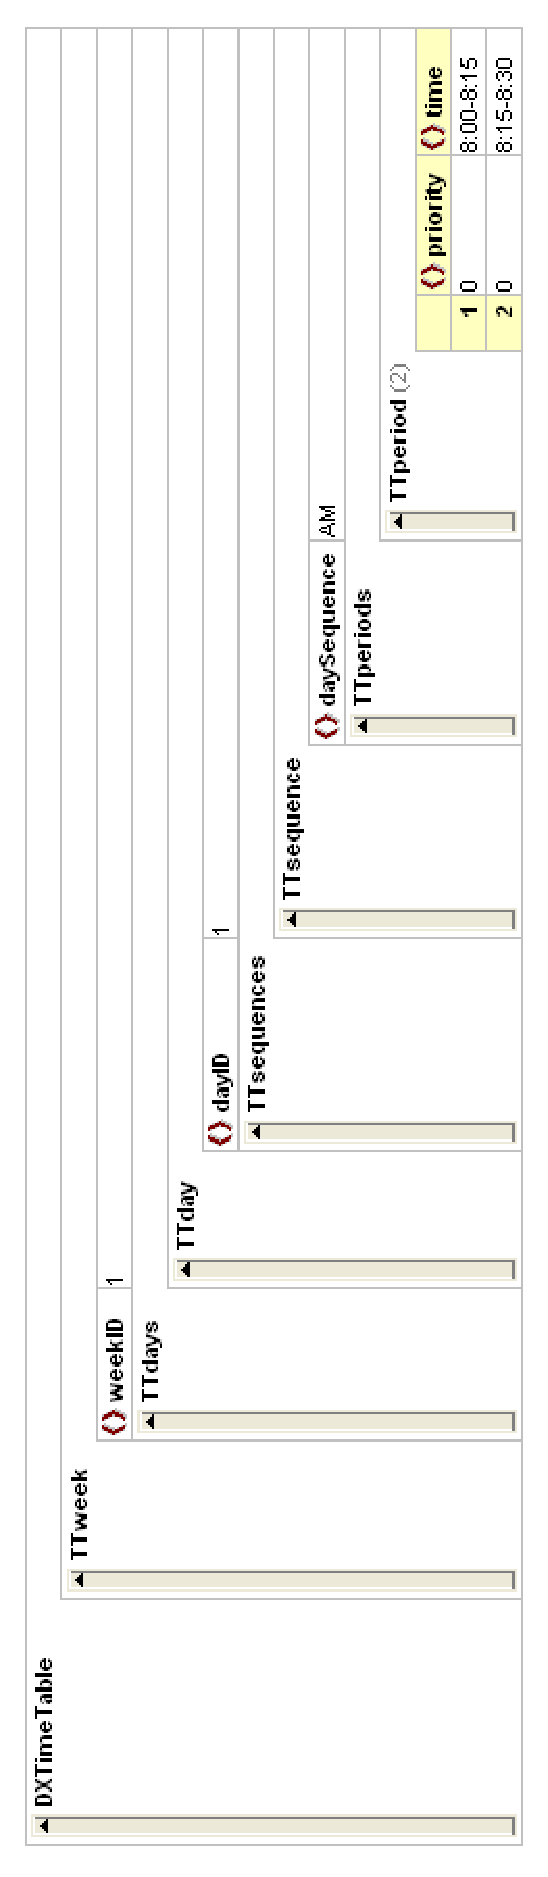
\includegraphics[width=400pt]{Images/TTxmlModel.eps}
    \caption{Schema du fichier XML de la grille horaire}\label{xmltt}
  \end{center}
\end{figure}


\section{Mod�lisation de la grille horaire}

\subsection{Organisation hi�rarchique}\label{hierar}

La nouvelle structure de la grille horaire de \diamant{} se pr�sente sous une forme hi�rarchique avec � son sommet la grille horaire compl�te et � la base les p�riodes (voir figure \ref{orgtt}), elle est d�crite comme suit:

\begin{itemize}
    \item Niveau 1: il correspond � la grille horaire complete et est constitu� de plusieurs �l�ments de niveau 2.\\

    \item Niveau 2: il correspond � l'ensemble des cycles de la grille horaire. Chaque �l�ment du niveau 2 (un cycle) est constitu� de plusieurs �l�ments de niveau 3.\\

    \item Niveau 3: il correspond � l'ensemble des jours d'un cycle. Chaque �l�ment du niveau 3 (une journ�e) est constitu� de plusieurs �l�ments de niveau 4.\\

    \item Niveau 4: il correspond � l'ensemble des s�quences d'une journ�e. chaque �l�ment du niveau 4 (une s�quence) est constitu� de plusieurs �l�ments de niveau 5.\\

    \item Niveau 5: il est l'entit� �l�mentaire de la grille horaire et il correspond � une p�riode dans laquelle devra �tre affect�e une activit�.
\end{itemize}


\begin{figure}[h]
  % Requires \usepackage{graphicx}
  \begin{center}
    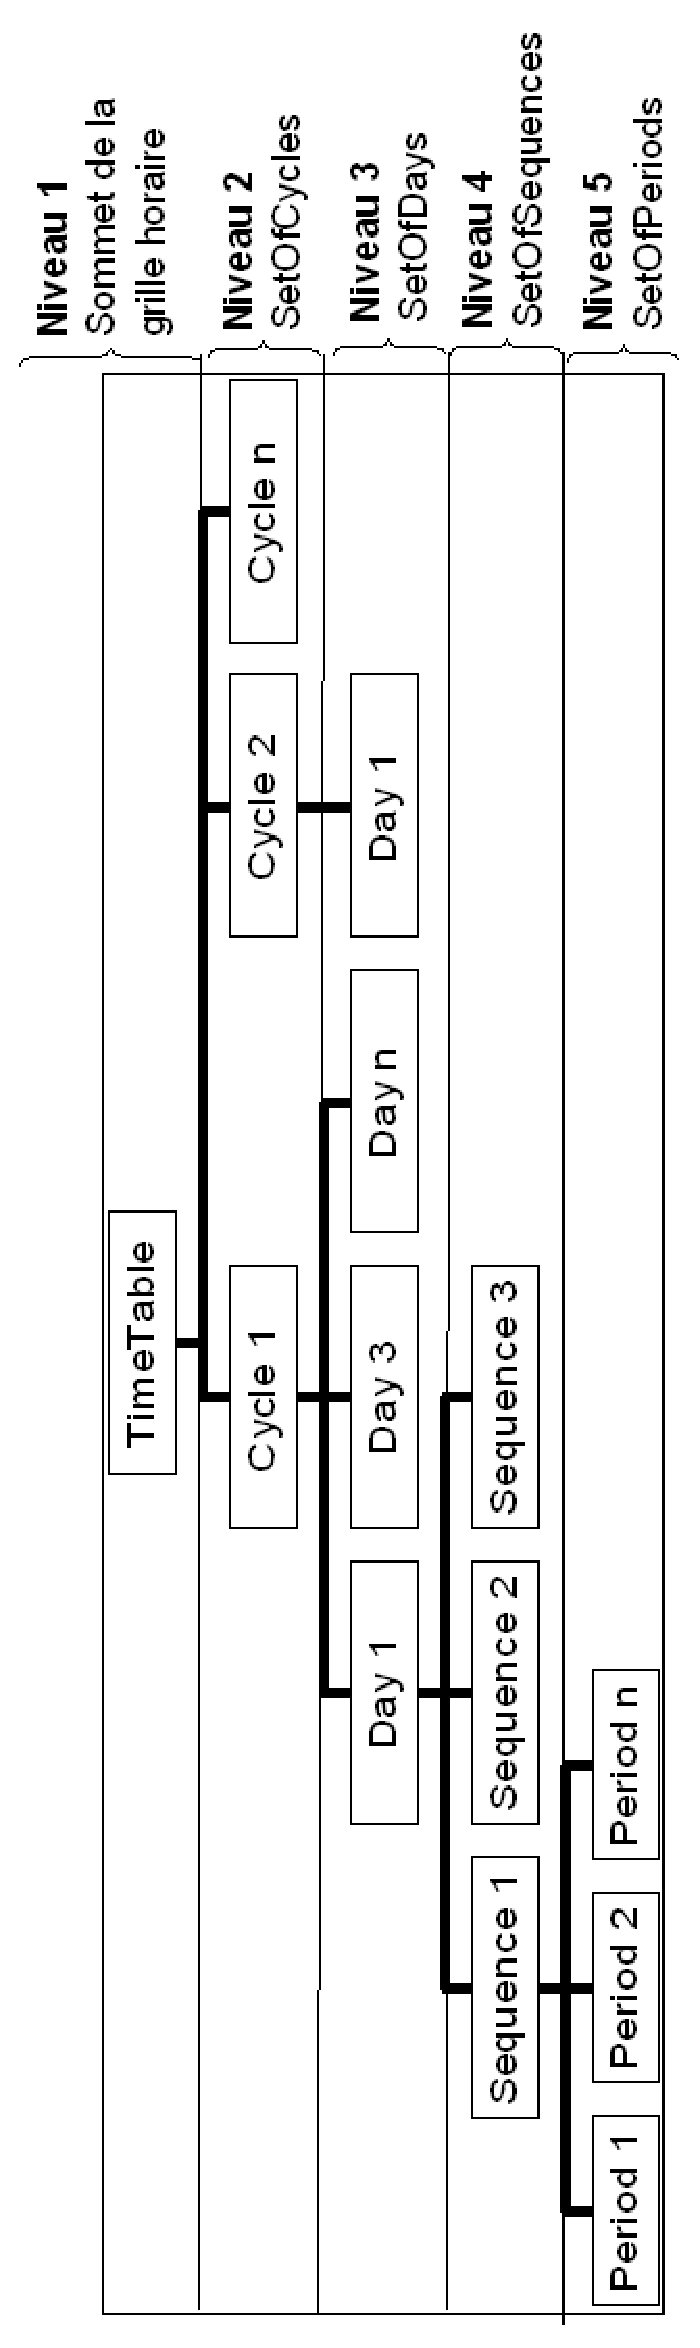
\includegraphics[height=6.0in,angle=-90]{Images/organigramme.eps}
    \caption{Schema hi�rarchique de la grille horaire}\label{orgtt}
  \end{center}
\end{figure}

\subsection{Mod�lisation objet}

Cette mod�lisation consiste � pr�senter le diagramme de classes de la grille horaire. Ce diagramme respecte la hi�rarchie d�crite � la section \ref{hierar} et est compos� de 3 types de classes (voir figure \ref{diagclass}):

\begin{itemize}
    \item Type 1: ce type ne concerne que la classe \emph{TTStructure} correspondant au sommet (niveau 1) de la grille horaire.\\

    \item Type 2: ce type concerne les classes fonctionnant comme des ensembles d'�l�ments (\emph{SetOfCycles, SetOfDays, SetOfSequences et SetOfPeriods}). Ces classes h�ritent de la classe \emph{SetOfResources} pour construire et manipuler leurs ensembles respectifs (voir l'article \emph{Chargement et traitement de donn�es � partir des fichiers textes }).\\
    \item Type 3: ce type concerne les classes fonctionnant comme des �l�ments d'ensembles (\emph{Cycle, Day, Sequence et Period}). Ces classes h�ritent de la classe \emph{DXObject} afin de pouvoir �tre int�gr�es � leurs ensembles respectifs.
\end{itemize}

\begin{figure}[h]
  % Requires \usepackage{graphicx}
  \begin{center}
    \includegraphics[width=450pt]{Images/dTimetable.eps}
    \caption{Diagramme de classes de la grille horaire}\label{diagclass}
  \end{center}
\end{figure}

\section{Avantages et limites de cette architecture}


%\part{Une partie}
%\include{revue}
%\include{theorie}

%\part{Derni�re partie}
%\chapter{Conclusion}

Bla bla bla bla bla.

Bla bla bla bla bla.


%\appendix
\chapter*{Glossaire}

Bla bla bla bla bla.

Bla bla bla bla bla.

\chapter*{Index}

A
AAA
ABC.

B
Bla bla bla bla bla.

%\include{formules}
\end{articleDX}
\end{document}
